\chapter {Ruolo del Videogame e Stato dell'Arte}
\label{chap:gaming_layer}

\section{Gaming Layer}

\subsection{Statistiche ed Evoluzione}

Una delle forme di intrattenimento più famose e usate al giorno d'oggi sono i videogame. Secondo i dati esposti nel report ESA 2014, l'età media dei videogiocatori è di 31 anni, e il 48\% di questi è di sesso femminile \cite{esareport-stats}.
Il numero di donne sopra i 50 anni che giocano ai videogame è aumentato del 32\% dal 2012 al 2013, in generale i gamer adulti hanno giocato per una media di 16 anni (nel dettaglio, gli adulti maschi hanno una media di 18 anni mentre le donne arrivano a 13) \cite{seriousgamingementor}.

\begin{figure}[h]
\centerline{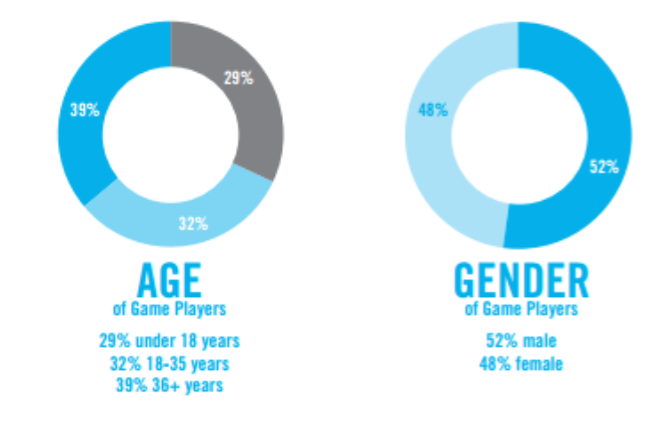
\includegraphics[scale=0.45]{images/statoarte/statsgamers.png}}
\caption{Statistiche sui videogiocatori.}
\label{fig:statsgamers}
\end{figure}

All'età di 21 anni, una persona abituata a giocare ai videogame, avrà già collezionato più di 10.000 ore di gioco, il che corrisponde a 40 ore a settimana per 5 anni, stesso tempo che un normale studente dedica alla scuola superiore \cite{seriousgamingementor}.

Questa situazione non sarebbe stata possibile anni fa, quando le reti di comunicazione non erano ancora così presenti nella vita quotidiana delle persone, le quali hanno quindi catalizzato la diffusione della cultura del videogame. Un altro fattore, che ha dato una spinta alla diffusione dei videogame, è certamente la presenza dei Social Network (come Facebook), i quali facilitano la diffusione dei cosidetti giochi ``virali'', cioè quei giochi che, fra le varie meccaniche, ne hanno una che prevede la diffusione del gioco tramite passaparola dei giocatori, i quali traggono spesso dei vantaggi dal fare questa azione (per esempio il bonus di 1 vita extra per il gioco Candy Crash Saga). E' quindi innegabile il potenziale divulgativo che possiede un videogame.

Ma il videogioco non è solo una forma di intrattenimento, secondo molti ricercatori rappresenta qualcosa di più.
Come si afferma in un articolo del sito ``PsychCentral'' \cite{phychcentral}, i giochi Sparatutto tendono a migliorare le skill cognitive come la navigazione spaziale, il ragionamento, la memoria e la percezione. 
Altri giochi più strategici (come i giochi di ruolo, o i puzzle solving) tendono a far sviluppare skill come il problem solving, per non parlare del multitasking che viene costantemente messo a dura prova in moltissimi giochi di abilità.


Detto ciò, è ragionevole considerare il videogame come mezzo di apprendimento e miglioramento. Per grandissima parte dei giochi questo apprendimento è stata una conseguenza ``non prevista'' da parte degli sviluppatori, 
in quanto il core principale dei giochi è sempre stato il solo intrattenimento. Esiste però una categoria di giochi il cui obiettivo non è solamente l'intrattenimento, ma anche il trasmettere altri concetti, come l'educazione o l'informazione riguardo una certa tematica, o addirittura il fornire un training riguardo un certo ambito (fornendo quindi delle volte una vera e propria simulazione al giocatore). Questa categoria di videogame si chiama ``Serious Game''.

\subsubsection{Theory of Fun}

Accanto ai Serious Game, esiste un'altro metodo che si basa sui principi dei giochi, questa è la Gamification (per una distinzione dettagliata fra Gamification e Serious Game fare riferimento alla paragrafo \ref{sec:distinzioni}).

Un esempio di Gamification è stata l'installazione di una tastiera musicale sulla scalinata dell'uscita di una metropolitana. Le persone, attratte e divertite dalla musica prodotta dal loro passaggio sugli scalini, preferivano usare le scale tradizionali piuttosto che le scale mobili. Alla fine si è riscontrato un aumento del 66\% delle persone che hanno preferito le scale tradizionali a quelle mobili.

Un secondo esempio ha riguardato i bidoni dell'immondizia di un parco: sono stati installati dei sensori, che all'arrivo di un rifiuto al proprio interno, facevano partire il suono tipico di un oggetto che cade per centinaia di metri nel vuoto. Questa semplice installazione ha attratto la curiosità di molti passanti, i quali, incuriositi e ignari della parte artificiale di tutto ciò, buttavano i rifiuti dei dintorni pur di sentire di nuovo quello strano suono e capirne qualcosa in più.

Questi scenari sono stati creati per un concorso indetto da Volkswagen chiamato ``Theory of fun'', nel quale si afferma: ``Qualcosa di tanto semplice come il divertimento rappresenta il modo più semplice per migliorare il comportamento delle persone in meglio''.

Sia i Serious Game che gli esperimenti di Gamification sono in linea con il nostro obiettivo, cioè spronare un certo pubblico ad interessarsi a luoghi di culto come i musei (nel nostro caso in particolare, il Museo del Cinema). Come abbiamo già detto, e rivedremo meglio nei prossimi capitoli, fra i due approcci si è scelto quello del Serious Game per lo sviluppo del progetto ``The Magic Lantern''.

\newpage

\subsection{Serious Game}

\subsubsection{Cosa Sono}
\label{sec:cosasono}

L'origine dei giochi a scopo formativo viene generalmente ricondotta alle simulazioni di guerra (''Kriegsspiel'') dell'esercito prussiano degli inizi del XVIII secolo.
Il termine Serious Game venne probabilmente usato la prima volta da Clark Abt, sviluppatore di giochi militari su computer, nel 1971. Nel suo libro Serious Game, il ricercatore statunitense fornisce anche una definizione dei giochi educativi, a prescindere dal supporto (digitale o real-world). Li descrive come giochi con un esplicito e ben strutturato scopo educativo, non pensati primariamente per il divertimento, senza però escluderlo \cite{wikiseriousgames}.
Nonostante la nascita di questi sia ormai datata, la loro diffusione sta aumentando soprattutto negli ultimi anni, grazie anche alle nuove tecnologie per lo sviluppo di videogame.

E' possibile identificare alcuni ambiti in cui i Serious Game agiscono, per esempio gli autori del sito \url{www.serious.gameclassification.com} \cite{seriousclass} hanno stabilito la seguente tassonomia: 

\begin{itemize}
\item Educative message broadcasting 
\item Informative message broadcasting
\item Marketing \& Communication message broadcasting
\item Subjective message broadcasting
\item Training
\item Goods trading
\item Storytelling
\item Licensed title
\end{itemize}

Sempre gli stessi autori hanno contribuito a varie conferenze e articoli scientifici sui Serious Game, disponibili sempre sul loro sito \cite{seriousclass}.


\subsubsection{Serious Game e altre forme di intrattenimento simili}
\label{sec:distinzioni}

Come già detto, il Serious Game non è l'unica forma di intrattenimento che si basa sul gaming (\myfig{\ref{fig:gameschema}}). 

\begin{figure}[h]
\centerline{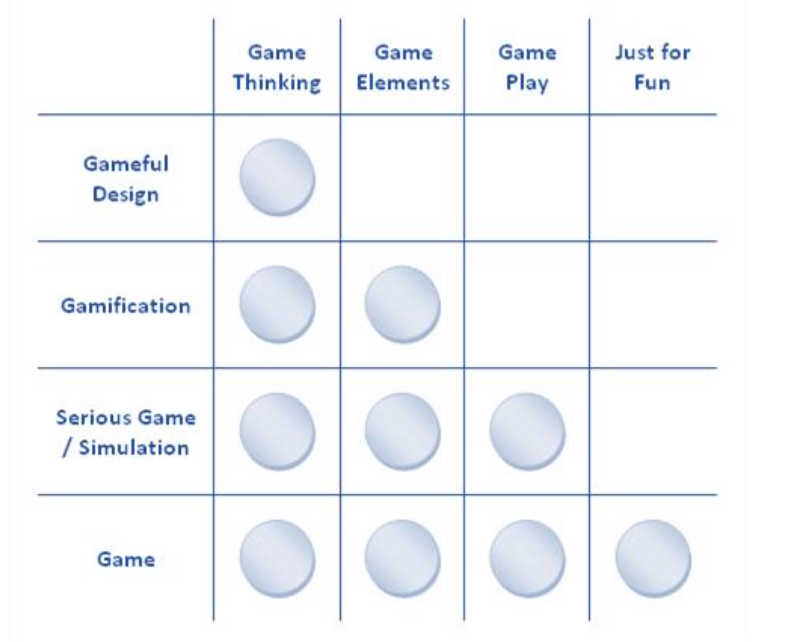
\includegraphics[scale=0.3]{images/statoarte/gameschema.png}}
\caption{Diversi approcci al gaming.}
\label{fig:gameschema}
\end{figure}

Possiamo distinguere 4 categorie:

\begin{itemize}
\item Gameful Design: ha una funzionalità spesso estetica, non ci sono elementi di gioco, ma il design ne ricorda il game thinking. Per esempio Twitter ha usato delle pagine molto particolari (al posto della tipica pagina con error 404) per casi in cui una pagina del sito non venga trovata \myfig{\ref{fig:gamefuldesignex}}.

\begin{figure}[h]
\centerline{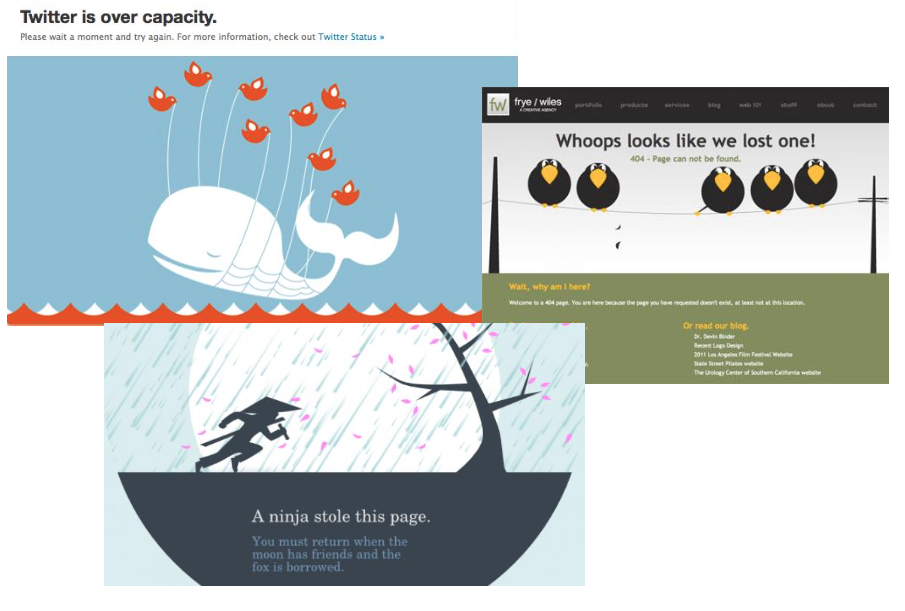
\includegraphics[scale=0.35]{images/statoarte/gamefuldesignex.png}}
\caption{Esempi di Gameful Design.}
\label{fig:gamefuldesignex}
\end{figure}

\item Gamification: contiene alcuni dei tipici elementi di gioco, come l'assegnazione di punti o il raggiungimento di livelli. Per esempio Dropbox ha creato una competizione fra gli atenei Universitari, dove l'obiettivo (per Ateneo) era raggiungere il numero più alto di iscritti. La ricompensa per gli studenti consisteva in GB gratis tramite il medesimo servizio di cloud \myfig{\ref{fig:gamefuldesignex}}.

\begin{figure}[b]
\centerline{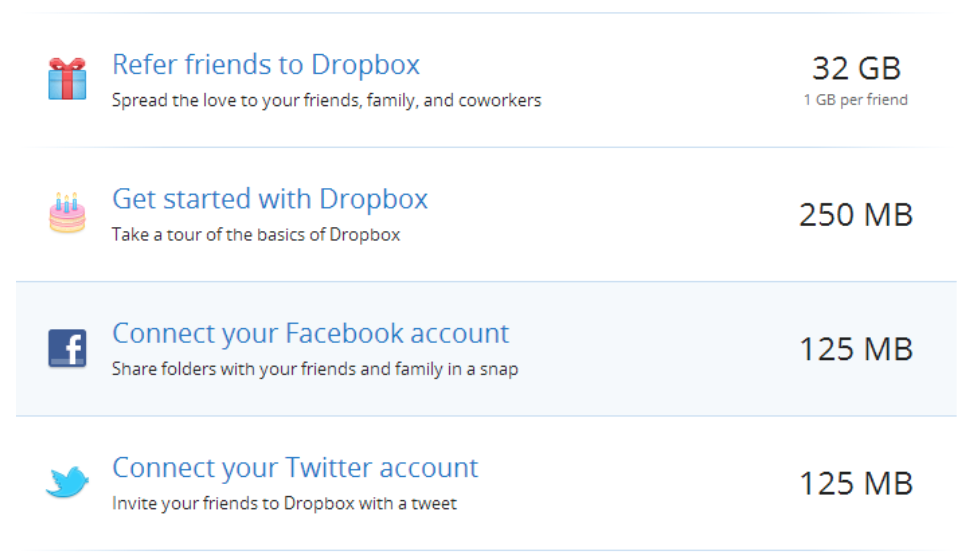
\includegraphics[scale=0.3]{images/statoarte/gamificationex.png}}
\caption{Esempio di Gamification.}
\label{fig:gamificationex}
\end{figure}

\item Serious Game: possiede tutte le caratteristiche di un videogame, il cui scopo però non è il solo divertimento. Per esempio, un Serious Game chiamato Dragon Box, si propone di insegnare le equazioni a dei bambini tramite dei rompicapo \cite{dragonboxhome}.


\item Game: sono i tipici videogame il cui obiettivo è solamente divertire e intrattenere il pubblico.
\end{itemize}

Il nostro prodotto si classifica come Serious Game in quanto presenta meccaniche pure di un videogame, quali platoform e rompicapo (che vedremo nel capitolo \ref{chap:game_design} sul Game Design), ma in più ha lo scopo di incuriosire il pubblico verso la tematica del pre-cinema.

\newpage

\subsubsection{Approccio Esperienziale}
\label{sec:seriousgameesp}

Come afferma Wikipedia \cite{wikiseriousgames}, non esiste una teoria uniforme sulla pedagogia dei Serious Game. Se in passato i giochi erano basati sulla psicologia comportamentale, come ad esempio nel gioco Mathblaster  \cite{mathblaster}, 
oggi gli sviluppatori di videogiochi educativi attingono da vari modelli pedagogici e particolare importanza ha assunto l'apprendimento esperienziale che parte dal presupposto che le informazioni 
e le sensazioni vissute rimangono fortemente impresse e permettono in questo modo al giocatore di affinare percezione, attenzione e memoria favorendo modifiche comportamentali attraverso il learning by doing (''imparare facendo'').

Uno dei punti di forza che ha il videogame nel fattore apprendimento consiste nella semplice interazione che si richiede all'utente. Come si può apprendere dalla relativa pagina su Wikipedia \cite{apprendimentoesperienziale}, questo modello di apprendimento si chiama esperienziale, e come suggerisce il nome, si basa sull'esperienza, sia essa cognitiva, emotiva o sensoriale. Il processo di apprendimento si realizza attraverso l'azione e la sperimentazione di situazioni, compiti, ruoli in cui il soggetto, attivo protagonista, si trova a mettere in campo le proprie risorse e competenze per l'elaborazione e/o la riorganizzazione di teorie e concetti volti al raggiungimento di un obiettivo. L'apprendimento esperienziale consente al soggetto di affrontare situazioni di incertezza sviluppando comportamenti adattivi e migliorando, nel contempo, la capacità di gestire la propria emotività nei momenti di maggiore stress psicologico. Consente inoltre di sviluppare le proprie abilità di problem solving, anche attraverso l'abilità creativa, e di far acquisire autoconsapevolezza mediante auto-osservazione ed etero-osservazione al fine di ridefinire eventuali atteggiamenti inadeguati e di valorizzare i comportamenti costruttivi. L'esperienza così acquisita diviene patrimonio di conoscenza del soggetto e costituirà il nuovo punto di partenza di ulteriori evoluzioni.

Questo approccio non è recente, e uno studio condotto a Washington \cite{vreduchristine} (risalente al 1996) ha raccolto dei dati interessanti sfruttando anche questa metodologia.
Questo studio mirava a capire quanto la realtà virtuale unita al videogioco potessero migliorare il grado di apprendimento dello studente, per esempio nel caso di un laboratorio di chimica. L'esperimento è stato condotto in varie modalità di apprendimento (solo le ultime 2 sfruttano l'approccio esperienziale): 

\begin{itemize}
\item semplice lezione,
\item lezione in videocassetta, 
\item gioco su pc, 
\item gioco con supporto di realtà virtuale.
\end{itemize}

Ciò che è stato dedotto tramite vari test effettuati sugli studenti è che l'apprendimento della lezione è in media superiore nei casi dove è richiesta una interazione (gioco pc, gioco in realtà virtuale). La statistica è stata a favore di queste categorie non solo per i test effettuati subito dopo i training, ma lo è stata anche e soprattutto per i test effettuati settimane dopo, ciò vuol dire che il ``fattore interazione'' tende a far apprendere stimolando non solo la memoria a breve termine ma anche quella a lungo termine.

Un altro fattore, molto affine all'approccio esperienziale, che rientra fra le caratteristiche dei giochi, è il ``trial-and-error'' come metodo per il problem-solving. Il trial-and-error \cite{trialanderror} ha varie caratteristiche: 

\begin{itemize}
\item Solution-oriented: questo approccio non cerca di capire perché una soluzione funzioni, ma si basa sul fatto che questa sia una soluzione;
\item Problem-specific: non si cerca di generalizzare una soluzioni ad altri problemi;
\item Non-optimal: si trova in genere una soluzione, non la soluzione migliore;
\item Needs little knowledge: questo metodo è perfetto soprattutto se si ha poca o nessuna conoscenza riguardo un ambito.
\end{itemize}

Dei famosi utilizzi di questo approccio sono avvenuti in ambito medico, con la scoperta degli antibiotici per esempio \cite{trialanderror}. Oggigiorno questo approccio è praticamente alla base di ogni videogame, dove il giocatore si appresta a scoprire sempre qualcosa di nuovo, e grazie a questo approccio ci si sente liberi di poter fallire e riprovare serenamente, finché non si sarà appreso la ``lezione'', la quale può consistere nel capire la giusta sequenza di tasti per sconfiggere un nemico, ma può anche consistere nell'apprendere come condurre un'esperimento chimico in tutta libertà e sicurezza.

\newpage

%--------------------------
%--------------------------

\section{Stato dell'arte}
\label{chap:stato_dell_arte}

\subsection{Giochi di interesse per il nostro caso di studio}

Come già detto, il nostro caso di studio ha come obiettivo la diffusione di informazioni riguardanti il pre-cinema, allo scopo di attrarre l'attenzione dei più giovani verso questa tematica e con la speranza che una certa percentuale di questi voglia quindi approfondire le loro conoscenze visitando il Museo del Cinema di Torino.

Per raggiungere questi obiettivi, il game design originale del gioco ``The Magic Lantern'' prevedeva un gameplay diviso a metà fra i generi platform e puzzle (rompicapo). E' stato quindi condotto uno studio sullo stato dell'arte di videogame appartenenti a queste due categorie, oltre che appartenenti alla tipologia Serious Game. In particolare, ci si è concentrati su Serious Game di tipo ``Informative message broadcasting'', i quali hanno appunto lo scopo di diffondere un certo tipo di messaggio, nel nostro caso sarebbe appunto l'esistenza delle tecnologie appartenenti al pre-cinema e quindi la loro storia.

Vediamo quindi di analizzare i singoli giochi che sono stati ritenuti utili per il nostro studio.

%--------------------------

\subsection{Valiant Hearts}

Valiant Hearts è un Serious Game ambientato nella prima guerra mondiale, il cui scopo è, oltre che divertire il player, far scoprire all'utente vari dettagli riguardo quel particolare periodo storico.

Il gioco ha delle meccaniche di tipo platform/avventura e puzzle (rompicapo): 

\begin{itemize}
\item platform/avventura poiché il mondo è esplorabile (tramite porte, piattaforme etc) e poiché sono presenti dei collezionabili da raccogliere; 
\item rompicapo perché alcune sezioni richiedono la risoluzione di alcuni indovinelli per essere superate.
\end{itemize}

Vediamo nella \myfig{\ref{fig:vhgameplay}} uno screenshot del gameplay del gioco. 

\begin{figure}[h]
\centerline{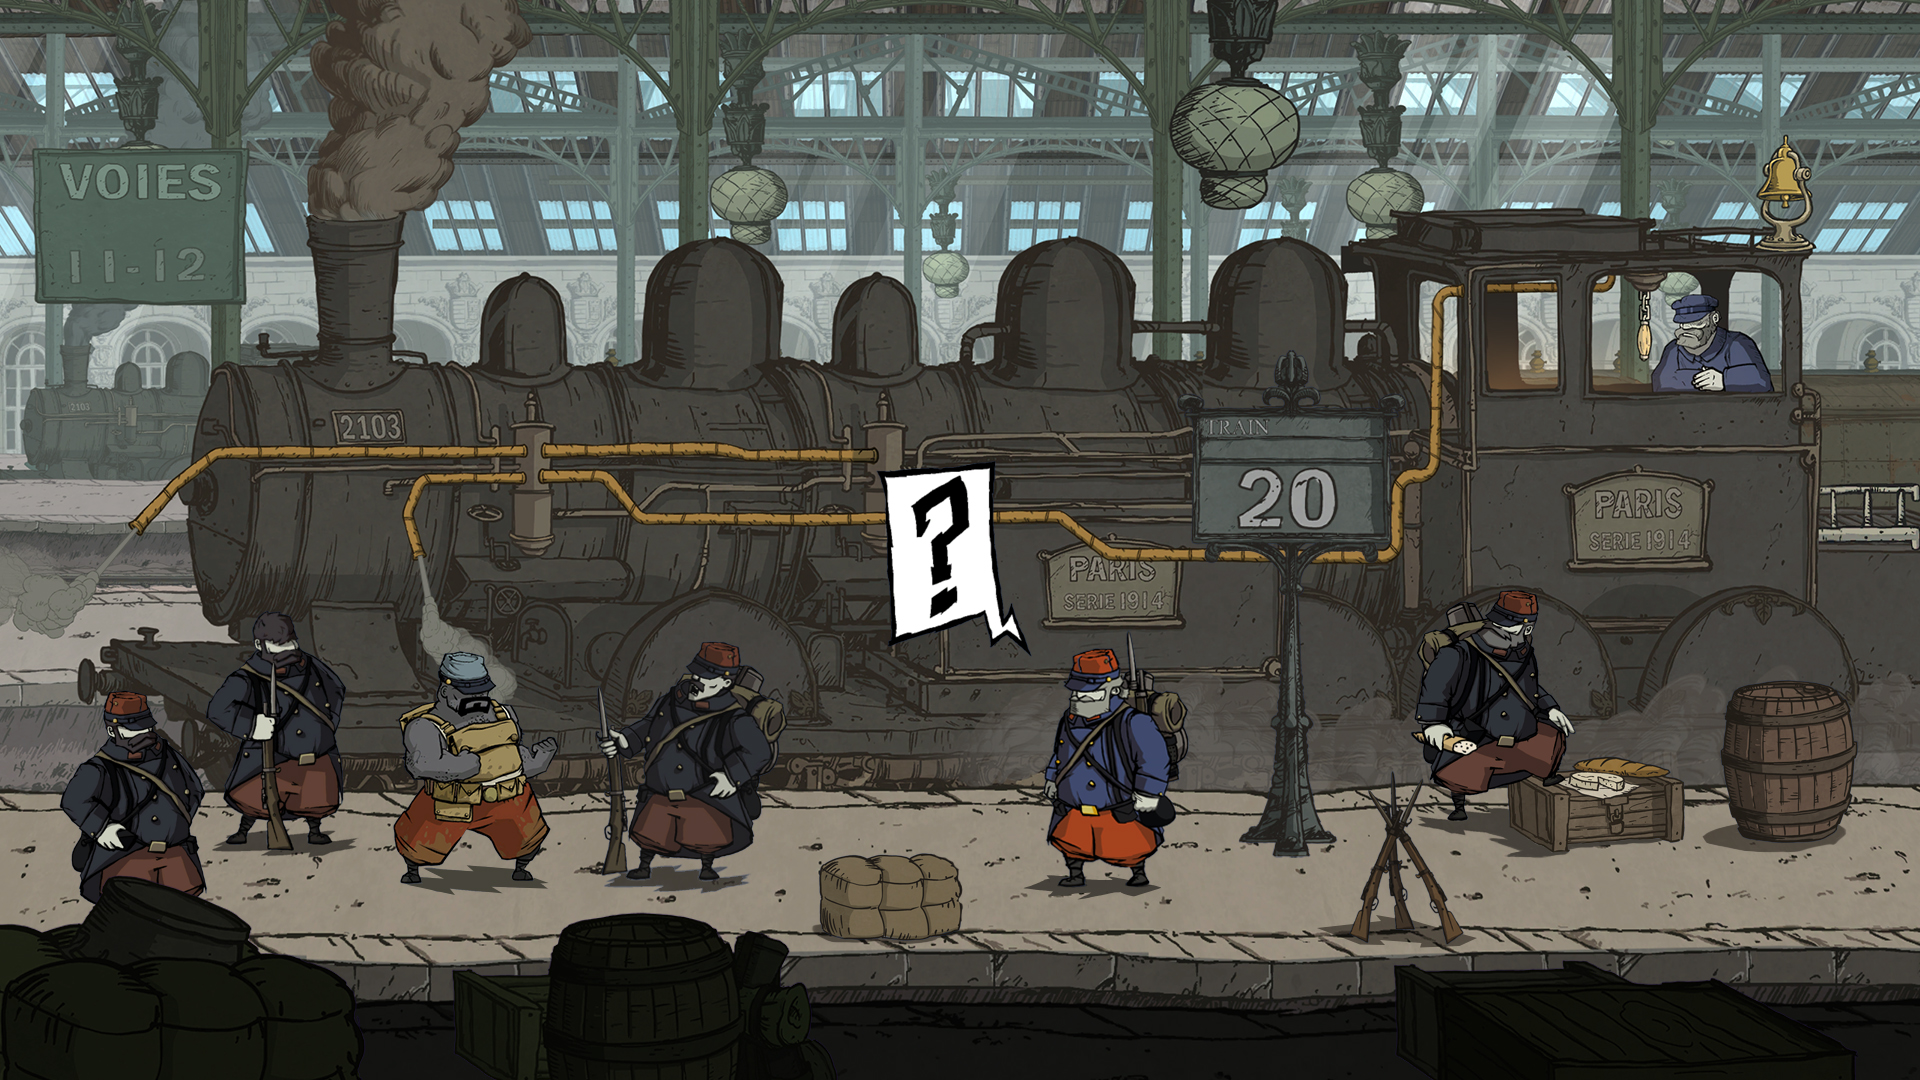
\includegraphics[scale=0.17]{images/statoarte/vhgameplay.jpg}}
\caption{Gameplay di Valiant Hearts.}
\label{fig:vhgameplay}
\end{figure}

Entrambe le tipologie di gioco favoriscono la parte Serious dell'esperienza:

\begin{itemize}
\item La parte platform aiuta in quanto ad ogni collezionabile preso viene sbloccata la corrispettiva scheda informativa, che spiega i dettagli storici riguardo quell'oggetto. Per esempio, la raccolta di una maschera a gas sblocca una scheda che narra dei primi attacchi batteriologici usati durante la prima guerra mondiale, oppure dopo aver raccolto una medaglietta da soldato dell'esercito, se ne spiegano i dettagli storici.
\item Alcune delle sezioni rompicapo sono collegate alle schede informative sbloccate, ciò invoglia il giocatore ad informarsi a riguardo. Per esempio durante un livello è presente una sezione con dei tubi che perdono gas letale, per superare questa sezione va risolto un indovinello. Proprio poco prima di questa sezione, l'utente ha avuto la possibilità di raccogliere l'oggetto maschera a gas e quindi di sbloccare la relativa scheda informativa.
\end{itemize}

Osservando la \myfig{\ref{fig:vhUIFacts}} è possibile capire come avvenga la fruizione di contenuti Serious del gioco. Una volta ottenuto un oggetto, si bloccherà il relativo ``Fatto'', leggibile da questa interfaccia, alla quale si può accedere in ogni momento di gioco.
La disposizione prevede: un menù di navigazione disposto in verticale sulla sinistra; una immagine rappresentativa del fatto storico posta in alto al centro; la descrizione del fatto storico in basso al centro.
\begin{figure}[h]
\centerline{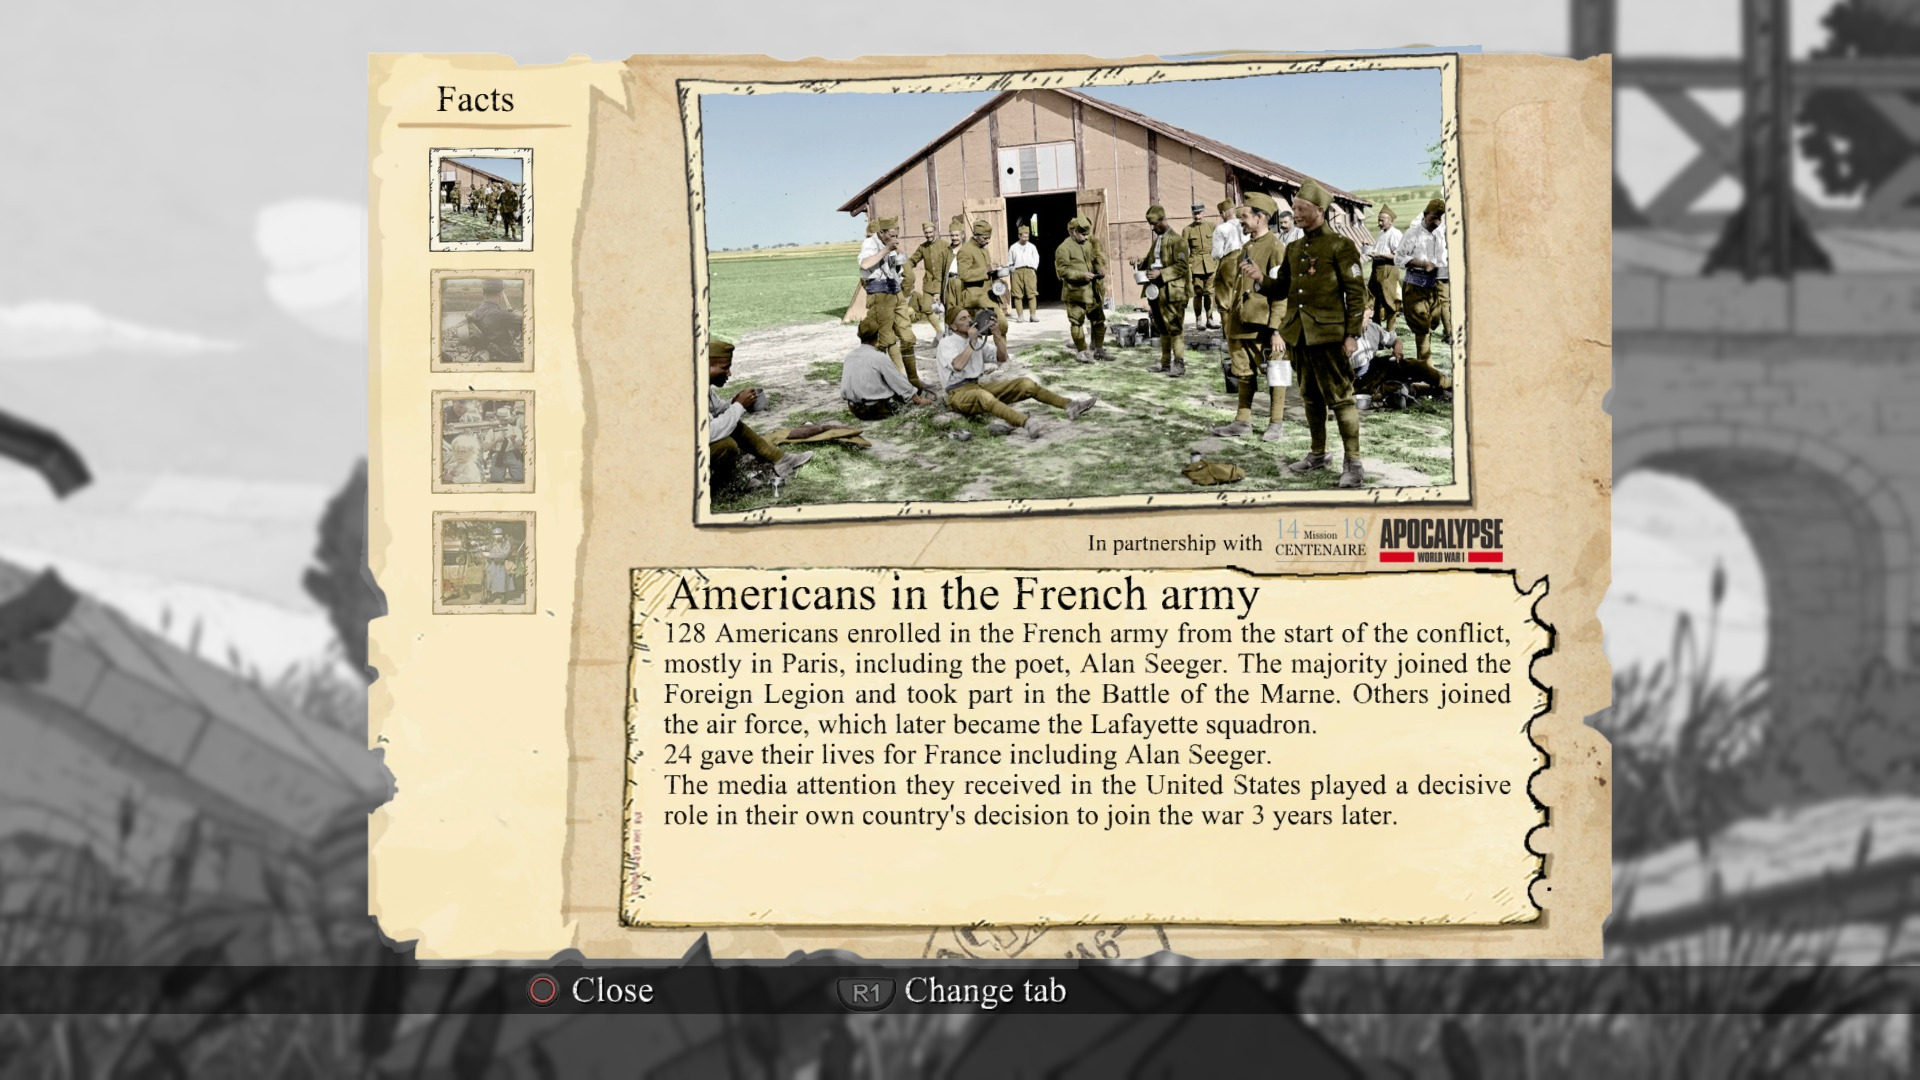
\includegraphics[scale=0.22]{images/statoarte/vhUIFacts.jpg}}
\caption{Menù dei contenuti Serious di Valiant Hearts.}
\label{fig:vhUIFacts}
\end{figure}

Gli sviluppatori (Ubisoft Montpellier) hanno scelto di produrre un gioco il cui scopo primario fosse quello del divertimento, lasciando libera scelta all'utente sulle modalità di approfondimento dei fatti storici correlati. Il gioco è stato prodotto per buona parte dei dispositivi in commercio: PlayStation3, PlayStation4, XboX360, XboxOne, PC, iOS, Android etc. Nonostante il genere platform, la giocabilità del titolo non risente troppo del porting su dispositivi mobili, questo anche perché non si richiede quasi mai all'utente una elevata maestria e coordinazione coi comandi, così da rendere il gioco mediamente facile e alla portata di tutti.

In conclusione, il gioco ha ricevuto ottimi feedback dalla critica, con voti molto alti come nel caso di IGN Italia (9/10) e Multiplayer.it (8/10) \cite{ignitalia} \cite{multiplayerit}. Ha inoltre vinto il premio speciale da ``Games for Change'' come gioco dell'anno per l'edizione 2014 \cite{gamesforchange}.

%--------------------------

\subsection{Never Alone}

Never Alone è un gioco dai principi molto simili a quelli di Valiant Hearts: l'obiettivo primario resta quello di intrattenere e divertire il giocatore, facendo nel frattempo scoprire informazioni riguardo la cultura Iñupiat.

Il gioco ha una forte connotazione platform e rompicapo, in quanto il giocatore dovrà superare il mondo posto sotto forma di piattaforme poste spesso ad altezze diverse. Il gameplay prevede l'utilizzo di due personaggi, una bambina e una volpe. Il giocatore potrà controllare l'una o l'altro, cambiando i comandi in qualsiasi momento. Gli sviluppatori hanno dato la possibilità di giocare in cooperativa locale, in modo tale da far controllare la bambina ad un player e la volpe all'altro player.
La meccanica proposta è piacevole e la difficoltà di gioco è nella media. La fruizione di contenuti Serious è data tramite dei video registrati appositamente per questo gioco (vedi \myfig{\ref{fig:videona}}), dove delle persone Iñupiat parlano riguardo le proprie usanze e miti storici. La visione dei video risulta essere piacevole e difficilmente stanca l'utente, in quanto la durata di ognuno è opzionale e ha una durata media di 1-2 minuti. La presenza di video agevola ancor di più l'utente riguardo l'apprendimento di questi contenuti extra, in quanto è risaputo che un utente medio difficilmente si ferma a leggere delle scritte a schermo, a meno che non si è obbligati per motivi vari (quali la comprensione della storia del gioco per esempio).

\begin{figure}[h]
\centerline{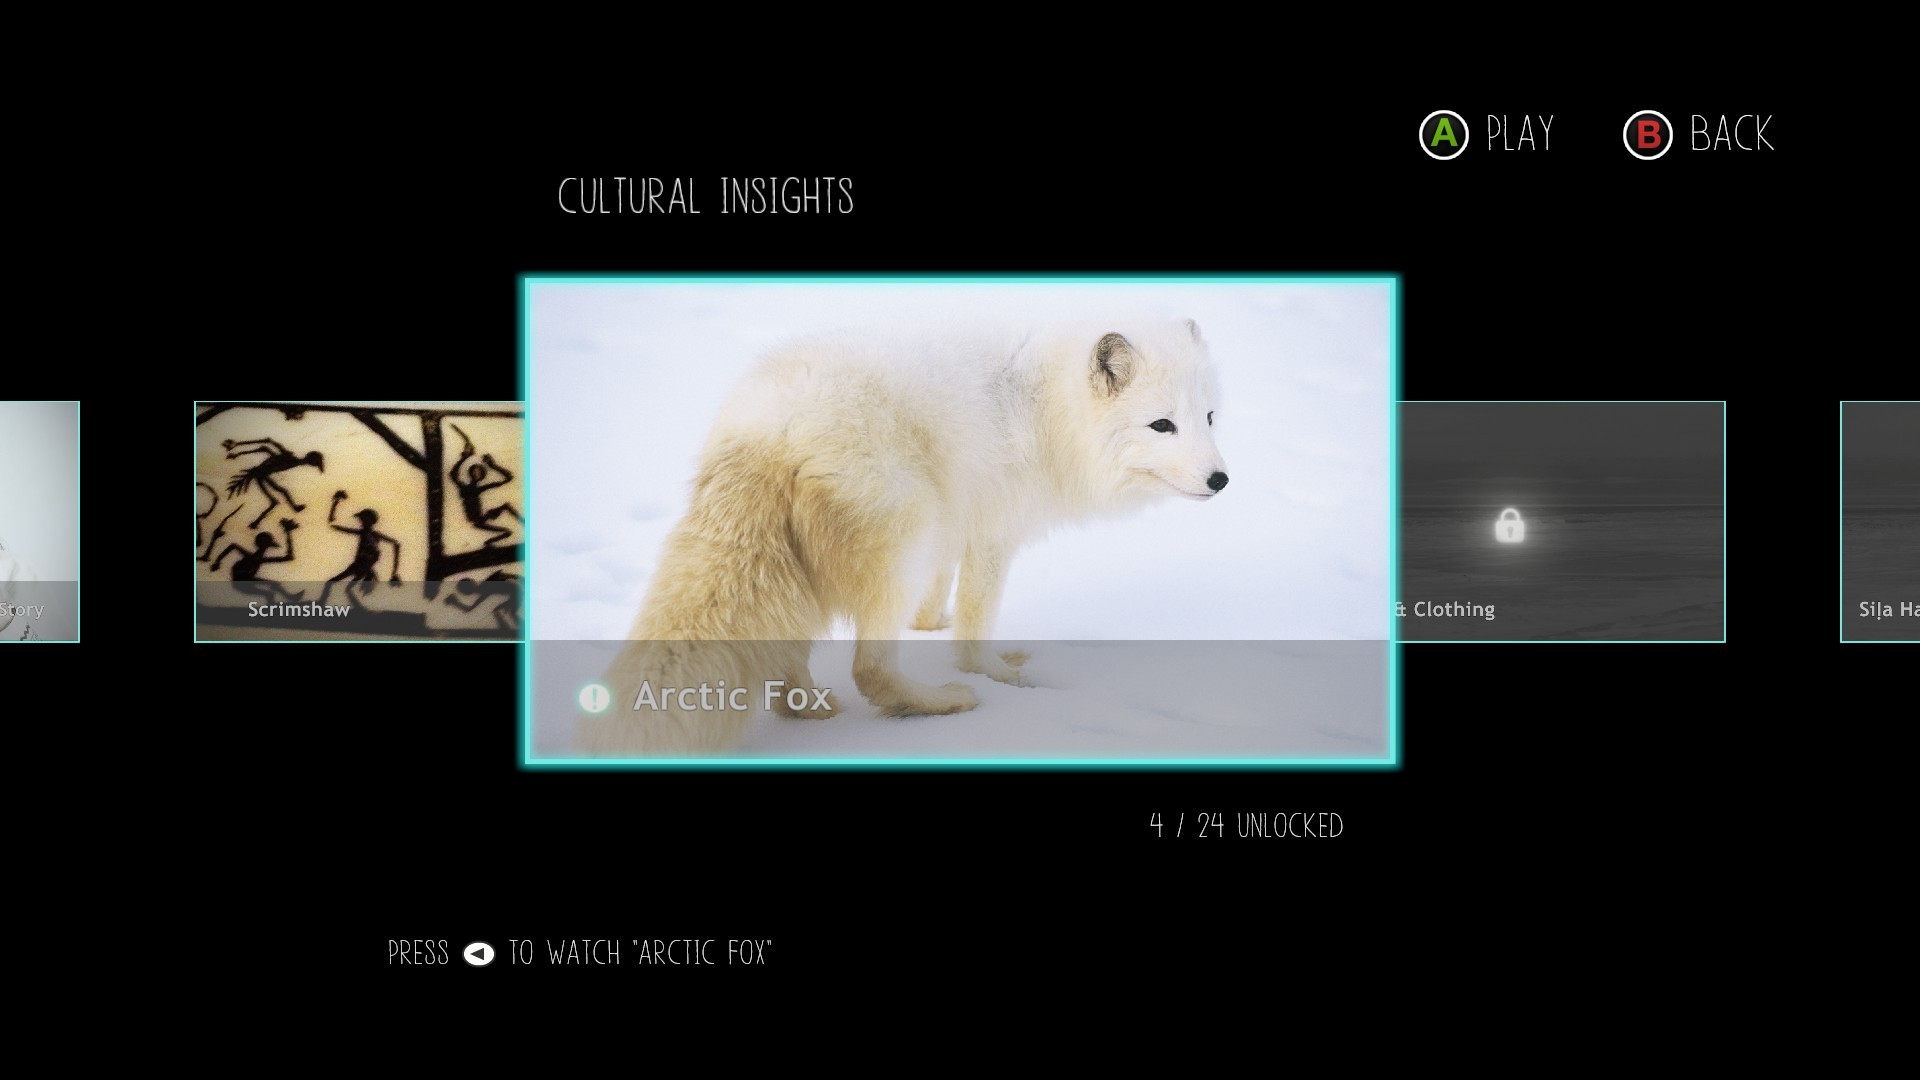
\includegraphics[scale=0.22]{images/statoarte/videona.jpg}}
\caption{Menù dei contenuti Serious di Never Alone.}
\label{fig:videona}
\end{figure}

Il gioco è stato sviluppato per PC, OS X, PlayStation3, PlayStation4, XboX360, XboxOne e Wii U. Come Valiant Hearts, anche Never Alone ha ricevuto ottime critiche, ed è stato premiato da ``Game for Changes'' come ``Most Impact'' e ``Game of the year''.


%--------------------------

\subsection{Super Mario}

Citiamo anche i giochi di Super Mario, in particolare modo riferendoci alle sue prime versioni (quindi titoli precedenti all'anno 1996, dove è comparso il primo Super Mario in 3D), in quanto sono state oggetto di studio riguardo le meccaniche platform 2D.

Ricordiamo che Super Mario è stato fra i primissimi giochi platform, cioè un gioco dove si salta da una piattaforma all'altra, spesso poste ad altezze diverse. Il gioco presenta anche una certa varietà di nemici, e le edizioni successive alla prima offrono anche un certo numero di ``power up'', cioè potenziamenti per l'avatar (per esempio la possibilità di sparare fiammelle dalla mano, in modo da uccidere i nemici anche da lontano e non per forza saltando loro addosso).
La principale difficoltà del gioco consiste nel coordinare salti e movimenti in base all'ambiente circostante, il giocatore mette quindi a dura prova i propri riflessi e tempismo durante il gameplay, il quale presenta una difficoltà di non poco superiore rispetto ai platform dei giorni nostri. I nemici presenti nel gioco sono vari, i più famosi sono i Goomba, i quali semplicemente vagano nel mondo, senza curarsi della presenza del player, altri nemici invece sono in grado di lanciare oggetti al giocatore, con lo scopo di ucciderlo.
E' stato particolarmente utile notare la gestione delle forze usate per il salto dell'avatar e di come quest'ultimo rimbalzi sopra i nemici dopo averli calpestati. La forza del salto, e quindi l'altezza massima raggiunta da Mario, è proporzionale alla durata della pressione del tasto A (usato appunto per saltare), quindi, brevi pressioni corrisponderanno a piccoli salti, lunghe pressioni invece produrranno il salto ad altezza massima. Inoltre, alcune versioni di Super Mario gestiscono anche la fase di atterraggio in base alla pressione del tasto A: in Super Mario World (1990)  per esempio, se la pressione del tasto continua anche dopo il raggiungimento del picco in altezza, la caduta risultava essere più lenta, non appena il tasto viene rilasciato si ha invece ha discesa rapida. Questo meccanismo è stato implementato per dare un maggior controllo al giocatore sulla precisione dei salti, in quanto meccanica fulcro del gameplay, la quale è spesso fondamentale per raggiungere punti particolari di gioco (come per esempio nemici in movimento).
In quasi tutti i Super Mario la gestione dei livelli gioco ha una struttura ad hub, cioè è presente una ``stanza centrale'' o mappa di riferimento, dalla quale accedere ai vari livelli.

\begin{figure}[h]
\centerline{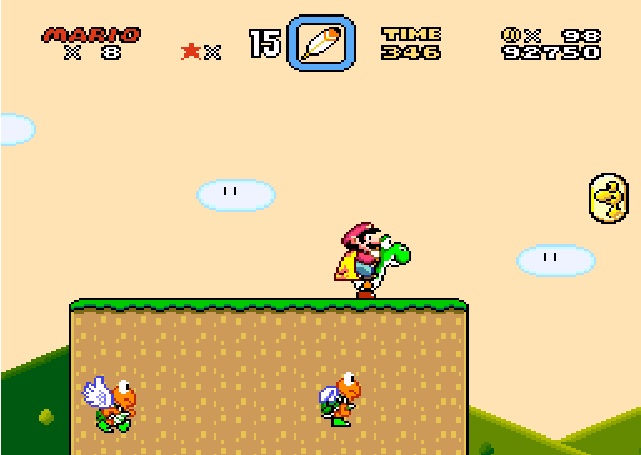
\includegraphics[scale=0.50]{images/statoarte/smwgameplay.jpg}}
\caption{Gameplay di Super Mario World.}
\label{fig:smwgameplay}
\end{figure}

Tutti i giochi di Super Mario sono disponibili per console Nintento. Negli ultimi anni, sono stati sviluppati dei titoli, sempre in 3D, ma con le vecchie meccaniche 2D, come per esempio ``New Super Mario Bros''.


%--------------------------

\subsection{Braid}

Braid è un gioco pubblicato nel 2008 e adotta delle meccaniche di gioco sia platform che puzzle. E' un gioco la cui meccanica predominante, oltre a quella dei salti, tipica dei platform, è quella di riportare indietro il tempo. Questo ``potere'', permette al giocatore di fare cose particolari fra cui risolvere indovinelli anche non banali. Durante l'evoluzione degli scenari, cambieranno anche gli elementi con cui potrà interagire il giocatore, (elementi come chiavi e relativa porta), e alcuni di questi reagiranno in modo particolare alla gestione del tempo, offrendo nuovi spunti per gli indovinelli proposti nel gioco. A differenza dei Super Mario, la potenza di salto non dipende dalla durata della pressione del relativo tasto, ma piuttosto ha una potenza standard. Anche qui i nemici possono essere uccisi tramite un salto sulla testa e questi uccidono il player per qualsiasi altro tipo di contatto. Ogni livello presenta un certo numero di collezionabili, i quali rappresentano i pezzi di un puzzle per un determinato ``mondo di gioco'', una volta raccolti tutti i pezzi sarà possibile ri-assemblare il puzzle e scoprire parte della storia principale. Come Super Mario, anche Braid ha una struttura dei livelli ad hub, il quale è rappresentato da una casa con delle stanze e porte al proprio interno, quindi ogni porta rappresenta l'accesso ad un mini mondo. In ogni stanza presente nella ``casa hub'' è presente un quadro raffigurante il puzzle da ricomporre coi pezzi raccolti nel mondo relativo a quella stanza.

I nemici presenti nel gioco sono in genere di 2 tipi:

\begin{itemize}
\item nemici stupidi: tendono a camminare in una direzione, e cambiare direzione nel caso si tocchi un muro (quindi nemici dalle caratteristiche simili ai Goomba di Super Mario);
\item nemici con carica: graficamente rappresentati con dei conigli, questi compaiono all'improvviso e dopo una breve carica, puntano il player con lo scopo di ucciderlo toccandolo.
\end{itemize}

\begin{figure}[h]
\centerline{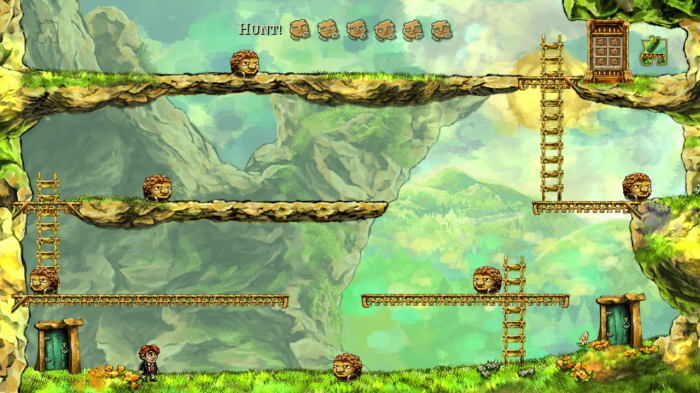
\includegraphics[scale=0.5]{images/statoarte/bgameplay.png}}
\caption{Gameplay di Braid.}
\label{fig:bgameplay}
\end{figure}

Il finale di gioco è sbloccato dopo che tutti i puzzle nei quadri sono stati riassemblati, a quel punto nella ``casa hub'' viene sbloccata una camera contenente il mondo finale.
Sono inoltre presenti nei vari livelli dei collezionabili segreti, i quali sono tutti molto difficili da notare. Se collezionati tutti, viene sbloccato un finale segreto alternativo.


%--------------------------

\subsection{The swapper}

The Swapper è un gioco puzzle-platform, rilasciato per varie piattaforme, fra cui Windows, Mac OS X, Linux e console come PlayStation3 e PlayStation4. Si tratta di un gioco fantascientifico, dove il giocatore si trova abbandonato su una nave spaziale di ricerca, e qui scopre uno strano device che gli permette di creare copie di se stesso e tele-trasportare la sua coscienza in uno dei suoi cloni. Questa meccanica, che consente al giocatore di proiettare in qualunque punto del gioco (tranne per punti specifici) cloni di se stesso, da una componente puzzle enorme al gioco, difatti, i livelli sono pieni di enigmi da risolvere tramite lo sdoppiamento del giocatore. Quasi tutti si basano sulla pressione di un bottone al giusto momento, e sul raccoglimento di vari oggetti sparsi per i livelli.

\begin{figure}[h]
\centerline{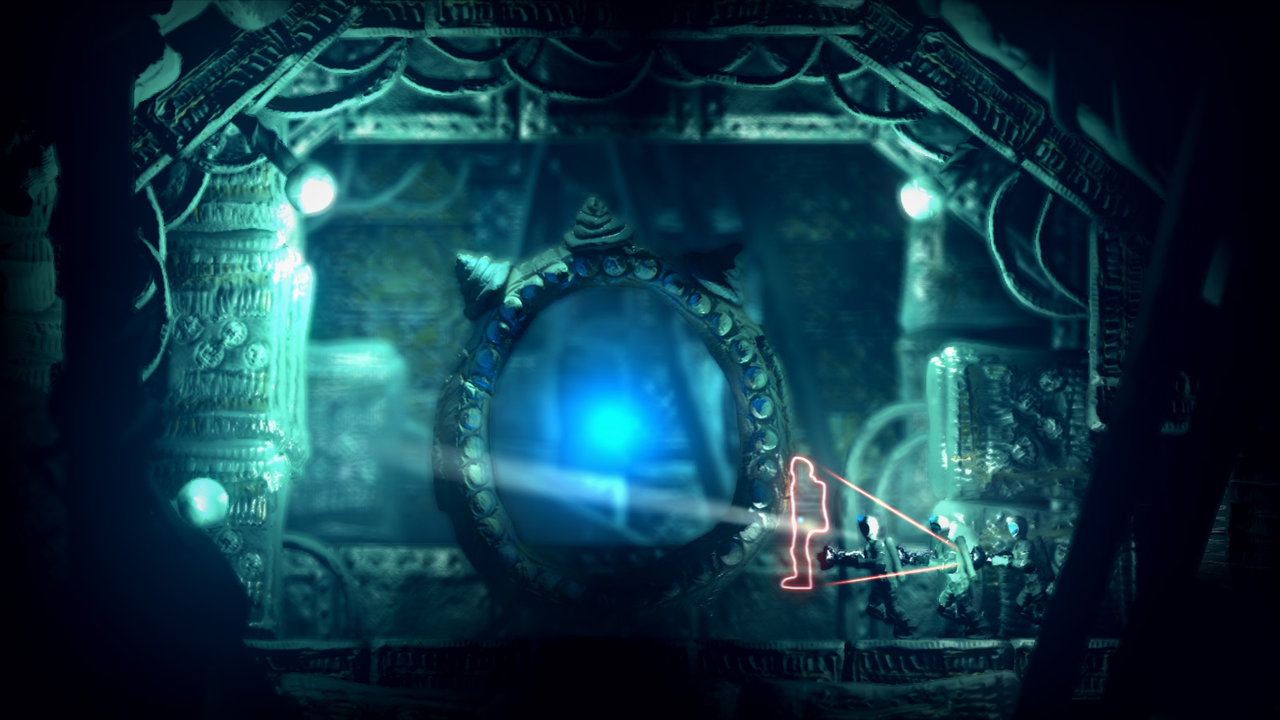
\includegraphics[scale=0.3]{images/statoarte/tsgameplay.png}}
\caption{Gameplay di The Swapper.}
\label{fig:pgameplay}
\end{figure}

%--------------------------

\subsection{Puppeteer}

Puppeteer è un gioco di tipo platform pubblicato nel 2013 per PlayStation3. Come si può notare in \myfig{\ref{fig:pgameplay}} sia la user interface che tutti i vari elementi di gioco, cercando di simulare uno spettacolo teatrale con dei burattini, difatti, è visibile il palcoscenico nella parte inferiore dello schermo e sono presenti anche i tendoni rossi sulle parti laterali e superiore. La narrazione, i dialoghi, i cambi di scena e tutti gli altri elementi richiamano benissimo le sensazioni che si provano durante uno spettacolo teatrale, il gioco risulta quindi essere un'opera molto artistica sotto questo punto di vista. Le meccaniche di gioco sono tante, in quanto, oltre al salto standard, sarà possibile fare un'azione speciale correlata al tipo di testa che si sta indossando, il cui numero si aggira intorno al centinaio (questo perché il personaggio ha perso la sua testa e la sostituisce con altre durante tutto il gioco). Ad un certo punto del gioco viene acquisito un altro potere, sottoforma di paio di forbici, le quali consentiranno di far arrampicare l'avatar su parti di mondo mentre queste vengono tagliate.

\begin{figure}[h]
\centerline{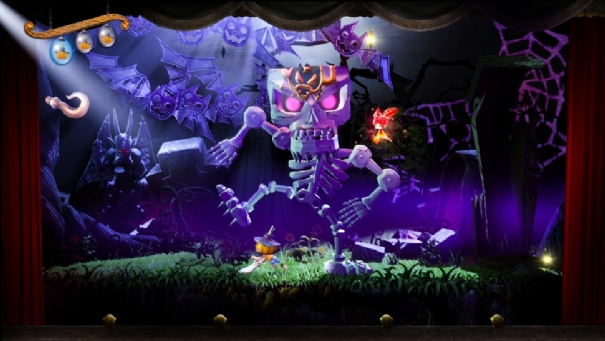
\includegraphics[scale=0.6]{images/statoarte/pgameplay.jpg}}
\caption{Gameplay di Puppeteer.}
\label{fig:pgameplay}
\end{figure}

Il gioco presenta una bassa difficoltà di superamento, difatti è un'opera adatta a tutti, soprattutto ad un pubblico infantile, il quale viene sicuramente affascinato da una grafica molto particolare che riesce decisamente a distinguersi dagli altri videogame, riuscendo a trasmettere al giocatore delle emozioni molto simili a quelle che darebbe un vero spettacolo di marionette.


%--------------------------

\section{Crescita dei Serious Game}

Esitono tanti altri Serious Game oltre a quelli citati finora (Valiant Hearts e Never Alone), e la loro diffusione è catalizzata da più fattori. 

Le ``Game Jam'' \cite{gamejamwiki} sono occasioni particolarmente efficaci per creare giochi del tutto innovativi. Questi sono degli eventi dalla durata media di 2-3 giorni che mettono assieme  persone dal diverso background, come game designer, sviluppatori, grafici e ogni altri tipo di figura interessata allo sviluppo dei videogame, al fine di creare dei giochi con una tematica in comune. Proprio fra il 2013-14 sono state organizzate delle Game Jam con tematiche Serious, grazie anche alla collaborazione con il progetto ``BOO-Games'' (progetto Europeo che mira alla sensibilizzazione riguardo lo sviluppo di Serious Game \cite{boogamesproject}\cite{boogamesprojecthome}). Una di queste Game Jam si è tenuta a Torino nel giugno del 2014 e ha avuto come tematica proprio l'informatica \cite{jamtoday}.

Un'altra comunità che sprona lo sviluppo dell'ambito Serious è ``Games for Change'' \cite{gamesforchange}, la quale organizza spesso eventi con talk di importanti figure del mondo videoludico per informare e sensibilizzare publisher, sviluppatori e insegnanti riguardo il potenziale dei Serious Game. Come già detto, è proprio ad eventi organizzati da "Games for Change" che giochi come Valiant Hearts e Never Alone hanno ricevuto importanti riconoscimenti.

Anche il Governo degli Stati Uniti d'America è attivo su questo fronte, e lo testimonia la scelta strategica di Barack Obama di investire milioni di dollari sull'ambito dell'education technology. Lo SBIR program (Small Business Innovation Research \cite{sbirprogram}) dell'istituto di Education Sciences darà più di un milione di dollari alle piccole aziende per la ricerca e lo sviluppo di prodotti commercializzabili per l'education technology. In reazione a ciò ci sono state varie proposte e sono nati giochi molto interessanti, come per esempio dei giochi riguardo le scienze naturali.


Adesso che abbiamo parlato dello stato dell'arte dei Serious Game e di altri giochi utili per i nostri studi, vediamo di affrontare meglio il nostro caso specifico.

\newpage
